\documentclass{beamer}

% --------------------------------------------------
% PAQUETES
% --------------------------------------------------
\usepackage[utf8]{inputenc}
\usepackage[T1]{fontenc}
\usepackage{amsmath, amssymb}
\usepackage{physics}
\usepackage{graphicx}
\usepackage{bm}

% --------------------------------------------------
% COLORES (ROJO Y BLANCO)
% --------------------------------------------------
\definecolor{uniRed}{RGB}{180,0,0}
\definecolor{lightGray}{RGB}{245,245,245}

\setbeamercolor{structure}{fg=uniRed}
\setbeamercolor{palette primary}{bg=uniRed, fg=white}
\setbeamercolor{palette secondary}{bg=uniRed!85, fg=white}
\setbeamercolor{palette tertiary}{bg=uniRed!70, fg=white}
\setbeamercolor{frametitle}{fg=white, bg=uniRed}
\setbeamercolor{title}{fg=white}
\setbeamercolor{normal text}{fg=black, bg=white}

% --------------------------------------------------
% TEMA
% --------------------------------------------------
\usetheme{Madrid}
\setbeamertemplate{navigation symbols}{}

% --------------------------------------------------
% INFORMACIÓN
% --------------------------------------------------
\title[Interpolación orbital]{Interpolación de Lagrange e integración numérica clásica\\
	aplicadas al análisis de trayectorias orbitales}
\author{Juan Carlos Celis Lozada}
\institute{Universidad de Pamplona \\ Programa de Física}
\date{\today}

% ==================================================
\begin{document}
	
	% --------------------------------------------------
	% 1. PORTADA
	% --------------------------------------------------
	\begin{frame}
		\titlepage
	\end{frame}
	
	% ==================================================
	% INTRODUCCIÓN
	% ==================================================
	
	% --------------------------------------------------
	% 2. CONTEXTO
	% --------------------------------------------------
	\begin{frame}{Introducción al problema}
		\begin{columns}
			\column{0.6\textwidth}
			\begin{itemize}
				\item La interpolación polinómica es fundamental en análisis numérico.
				\item Permite reconstruir funciones continuas desde datos discretos.
				\item Se emplea en problemas físicos y astrodinámicos.
			\end{itemize}
			
			\column{0.38\textwidth}
			\centering
			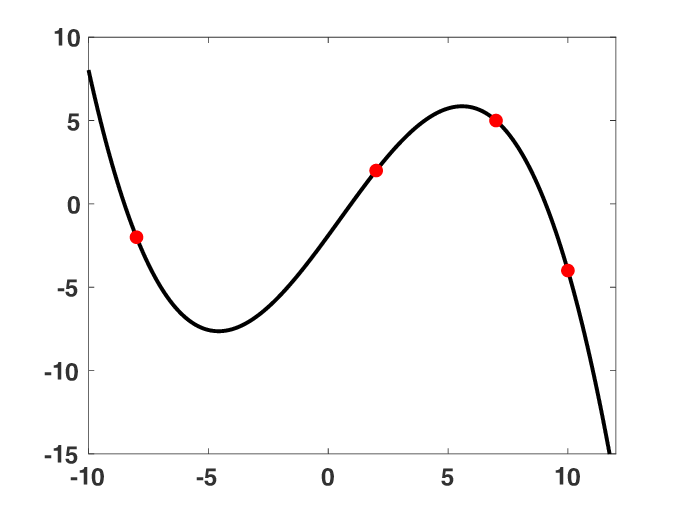
\includegraphics[width=\textwidth]{interpolación_general.png}
		\end{columns}
	\end{frame}
	
	% --------------------------------------------------
	% 3. PROBLEMA NUMÉRICO
	% --------------------------------------------------
	\begin{frame}{Introducción al problema}
		\begin{columns}
			\column{0.6\textwidth}
			\begin{itemize}
				\item La interpolación global puede presentar oscilaciones.
				\item Mallas equiespaciadas inducen el fenómeno de Runge.
				\item Su impacto en trayectorias orbitales no es trivial.
			\end{itemize}
			
			\column{0.38\textwidth}
			\centering
			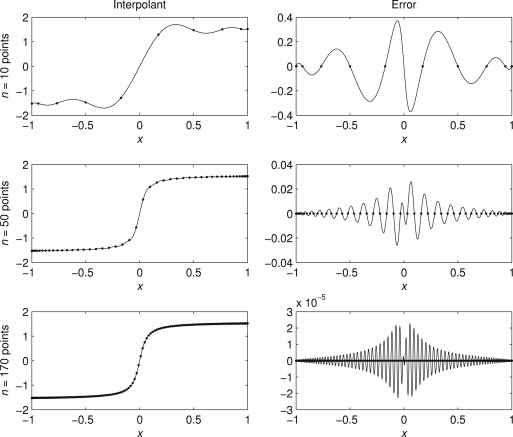
\includegraphics[width=\textwidth]{runge_teorico.jpg}
		\end{columns}
	\end{frame}
	
	% --------------------------------------------------
	% 4. MOTIVACIÓN
	% --------------------------------------------------
	\begin{frame}{Introducción al problema}
		\begin{columns}
			\column{0.6\textwidth}
			\begin{itemize}
				\item Las órbitas elípticas presentan regiones de alta curvatura.
				\item La interpolación se usa antes de integrar o derivar trayectorias.
				\item Es clave evaluar su efecto geométrico y numérico.
			\end{itemize}
			
			\column{0.38\textwidth}
			\centering
			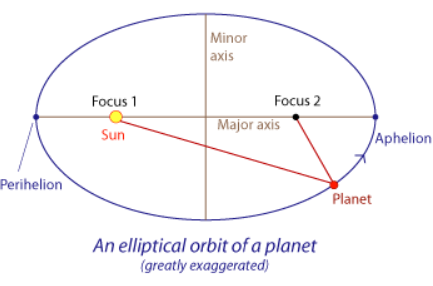
\includegraphics[width=\textwidth]{orbita_eliptica.png}
		\end{columns}
	\end{frame}
	
	% ==================================================
	% PLANTEAMIENTO
	% ==================================================
	
	% --------------------------------------------------
	% 5. MODELO ORBITAL
	% --------------------------------------------------
	\begin{frame}{Planteamiento}
		Órbita Kepleriana de referencia:
		\[
		r(\theta)=\frac{a(1-e^2)}{1-e\cos\theta}
		\]
		\[
		x(\theta)=r(\theta)\cos\theta, \quad
		y(\theta)=r(\theta)\sin\theta
		\]
	\end{frame}
	
	% --------------------------------------------------
	% 6. INTERPOLACIÓN
	% --------------------------------------------------
	\begin{frame}{Planteamiento}
		Interpolación polinómica de Lagrange:
		\[
		P(\theta)=\sum_{i=0}^{N-1} f(\theta_i)\,\ell_i(\theta)
		\]
		\[
		\ell_i(\theta)=\prod_{j\neq i}
		\frac{\theta-\theta_j}{\theta_i-\theta_j}
		\]
	\end{frame}
	
	% --------------------------------------------------
	% 7. METODOLOGÍA
	% --------------------------------------------------
	\begin{frame}{Planteamiento}
		\begin{itemize}
			\item Variación del número de nodos $N$.
			\item Variación de la excentricidad $e$.
			\item Evaluación del error geométrico.
			\item Comparación de integrales reales e interpoladas.
		\end{itemize}
	\end{frame}
	
	% ==================================================
	% RESULTADOS
	% ==================================================
	
	% --------------------------------------------------
	% 8. NODOS BAJOS
	% --------------------------------------------------
	\begin{frame}{Resultados: variación del número de nodos}
		\begin{columns}
			\column{0.48\textwidth}
			\centering
			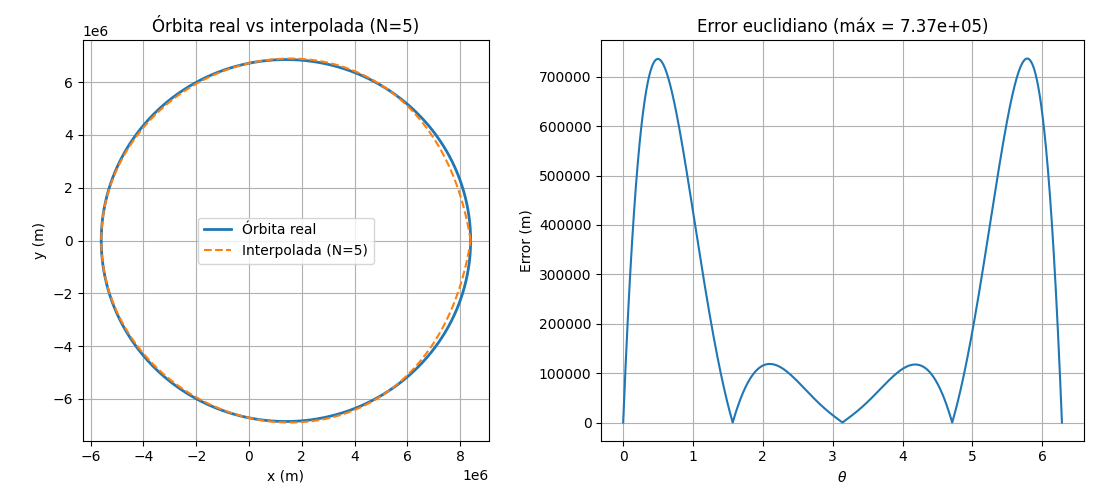
\includegraphics[width=\textwidth]{resultado1.png}
			\vspace{1mm}
			
			{\small $N=5$ nodos}
			
			\column{0.48\textwidth}
			\centering
			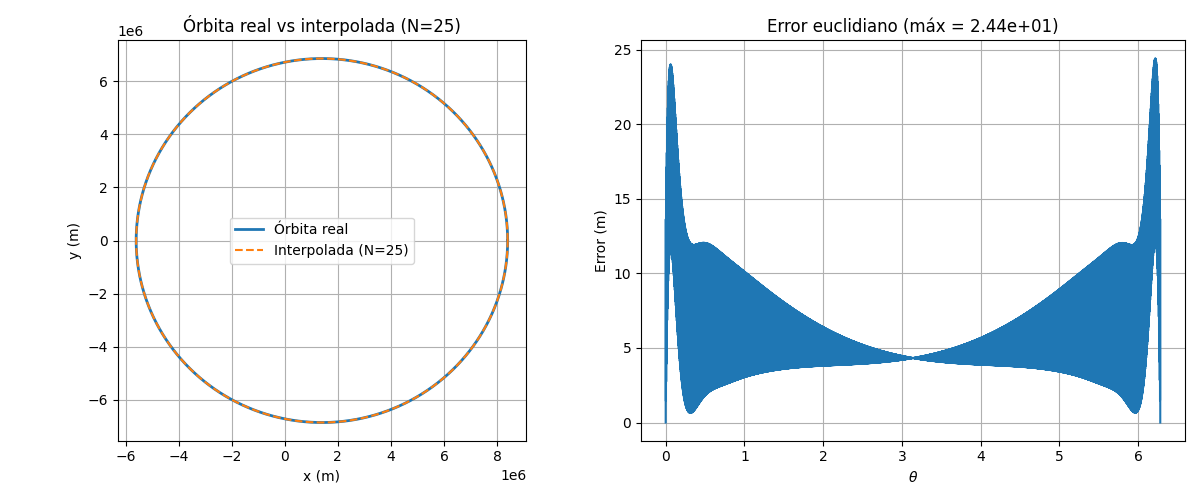
\includegraphics[width=\textwidth]{resultado11.png}
			\vspace{1mm}
			
			{\small $N=25$ nodos}
		\end{columns}
		
		\vspace{2mm}
		{\footnotesize Comparación entre reconstrucciones orbitales con distinto número de nodos.}
	\end{frame}
	
	% --------------------------------------------------
	% 9. NODOS ALTOS Y RUNGE
	% --------------------------------------------------
	\begin{frame}{Resultados: fenómeno de Runge}
		\centering
		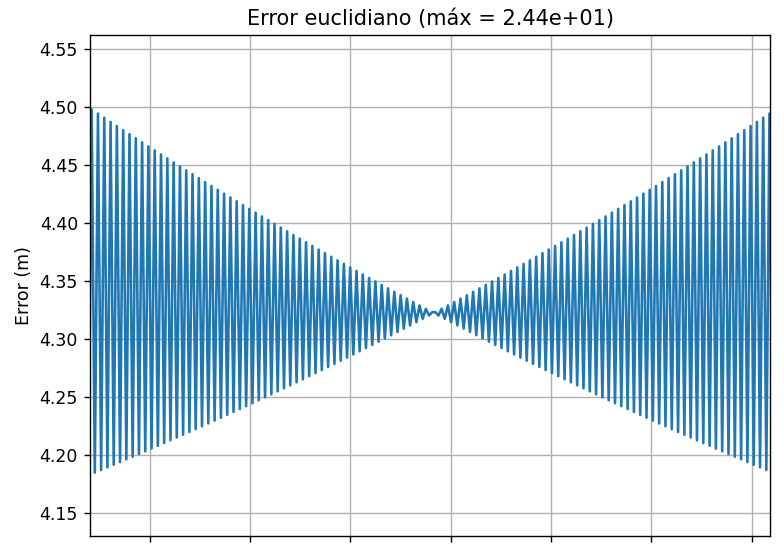
\includegraphics[width=0.75\textwidth]{runge.png}
		
		\vspace{2mm}
		Oscilaciones locales del error para $N$ grandes.
	\end{frame}
	
	% --------------------------------------------------
	% 10. VARIACIÓN DE EXCENTRICIDAD
	% --------------------------------------------------
	\begin{frame}{Resultados: excentricidad}
		\centering
		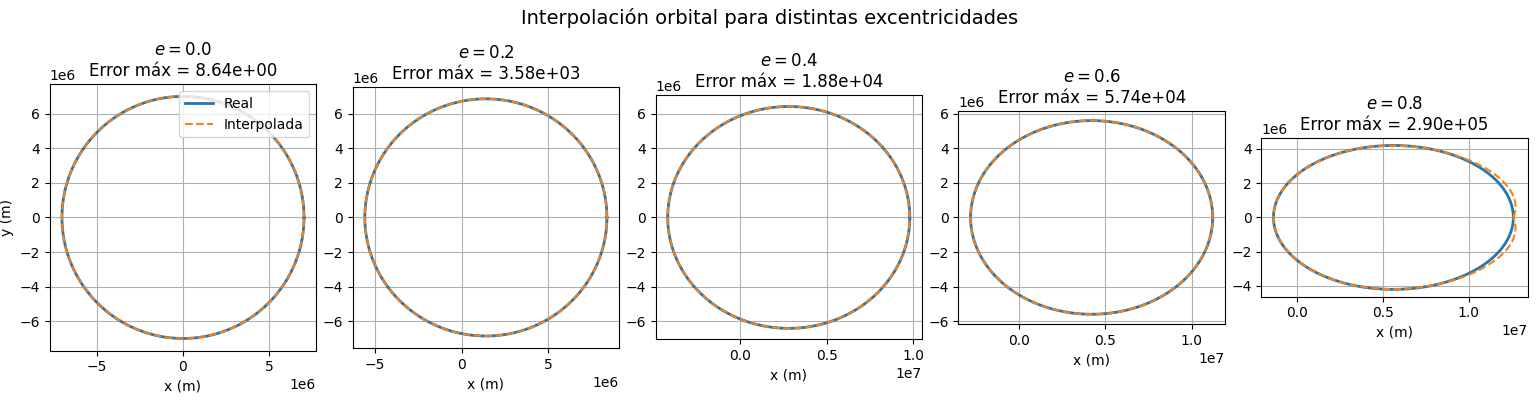
\includegraphics[width=0.8\textwidth]{Excentricidad.png}
		
		\vspace{2mm}
		El error aumenta con la excentricidad orbital.
	\end{frame}
	
	% --------------------------------------------------
	% 11. CASO e = 0.8
	% --------------------------------------------------
	\begin{frame}{Resultados: órbita excéntrica}
		\centering
		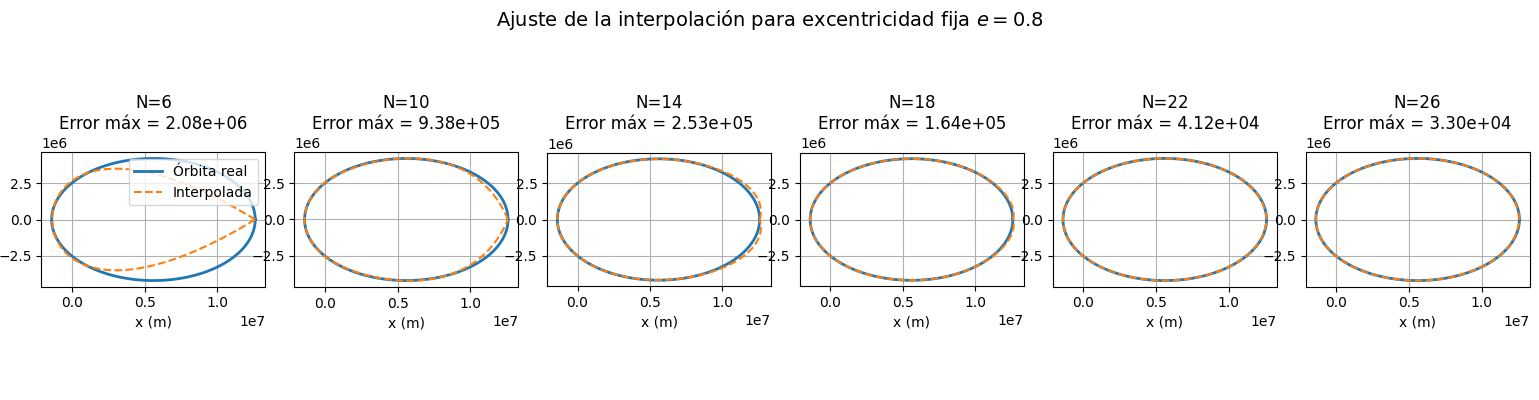
\includegraphics[width=0.8\textwidth]{excentricidad nodos.png}
		
		\vspace{2mm}
		Dependencia crítica del número de nodos para $e=0.8$.
	\end{frame}
	
	\begin{frame}{Resultados: integración numérica}
		\begin{columns}
			\column{0.55\textwidth}
			\begin{itemize}
				\item Se evaluó la integral radial
				\[
				I=\int_{0}^{2\pi} r(\theta)\,d\theta
				\]
				
				\item Se comparó la órbita analítica con la órbita interpolada.
				
				\item Se emplearon los métodos de Simpson y Gauss--Legendre.
				
				\item Las diferencias se mantienen del orden de $10^{4}$,
				con errores relativos menores al $0.1\%$.
			\end{itemize}
			
			\column{0.4\textwidth}
			\centering
			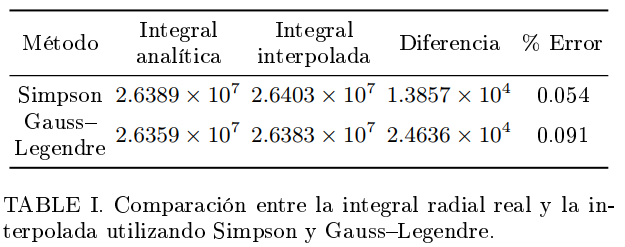
\includegraphics[width=\textwidth]{tabla_integracion.png}
			
			\vspace{1mm}
			{\footnotesize Tabla de comparación tomada del letter.}
		\end{columns}
	\end{frame}
	% ==================================================
	% CONCLUSIONES
	% ==================================================
	
	% --------------------------------------------------
	% 12. CONCLUSIONES
	% --------------------------------------------------
	\begin{frame}{Conclusiones}
		\begin{itemize}
			\item La interpolación de Lagrange depende de $N$ y de $e$.
			\item Las órbitas excéntricas amplifican errores geométricos.
			\item El fenómeno de Runge limita la interpolación global.
			\item Simpson y Gauss--Legendre son métodos robustos.
			\item La interpolación introduce un sesgo pequeño en integrales.
			\item Su uso es válido si se controla la discretización.
		\end{itemize}
	\end{frame}
	
	
\end{document}
